\chapter{Software}\label{cp:sw}

This chapter is a description of the developed software. It provides an overview of the architecture and the implementation. The projects GitHub page provides the full source code, setup instructions and Doxygen documentation \citep{Belinda2020}. %TODO: possibly attach the whole Doxygen documentation (latex format) in attachments"

The project is licensed under the GNU General Public License v2.0.

\section{Overview}
The application is split into the user interface (UI) and data processing. Each part runs in a thread and they are kept separated from each other. The data processing class is called \mintinline{cpp}{Processing} and the user interface class \mintinline{cpp}{Window}. 

The user interface is built with Qt, an open-source widget toolkit for creating graphical user interfaces. Additionally, the subset Qt Widgets for Technical Applications (Qwt) is used to display the acquired data.

The \mintinline{cpp}{Processing} class handles data acquisition and processing, sending notifications to the UI with instructions on what action to perform or what values to update.

\subsection{Class Diagram}
Figure \ref{fig:CD} shows a simplified class diagram of the application. It shows the Processing and Window classes in the middle with their most important attributes. 

The Processing class has a ComediHandler object to acquire data, the OBPDetection object implements the core algorithm described in \myref{cp:algo} and the Datarecord object saves the raw data to a file. The state of the application is stored in the ProcState enum.

The Window class holds all the UI components. The class diagram in figure \ref{fig:CD} only shows the high level components that are not directly from the Qt library. SettingsDialog and InfoDialog can be opened through the menu bar to access the configuration and get further information about the application. The two Plot objects are always visible, while the rest of the main window depends on the Screen enum.

\begin{figure}[ht]
\centering
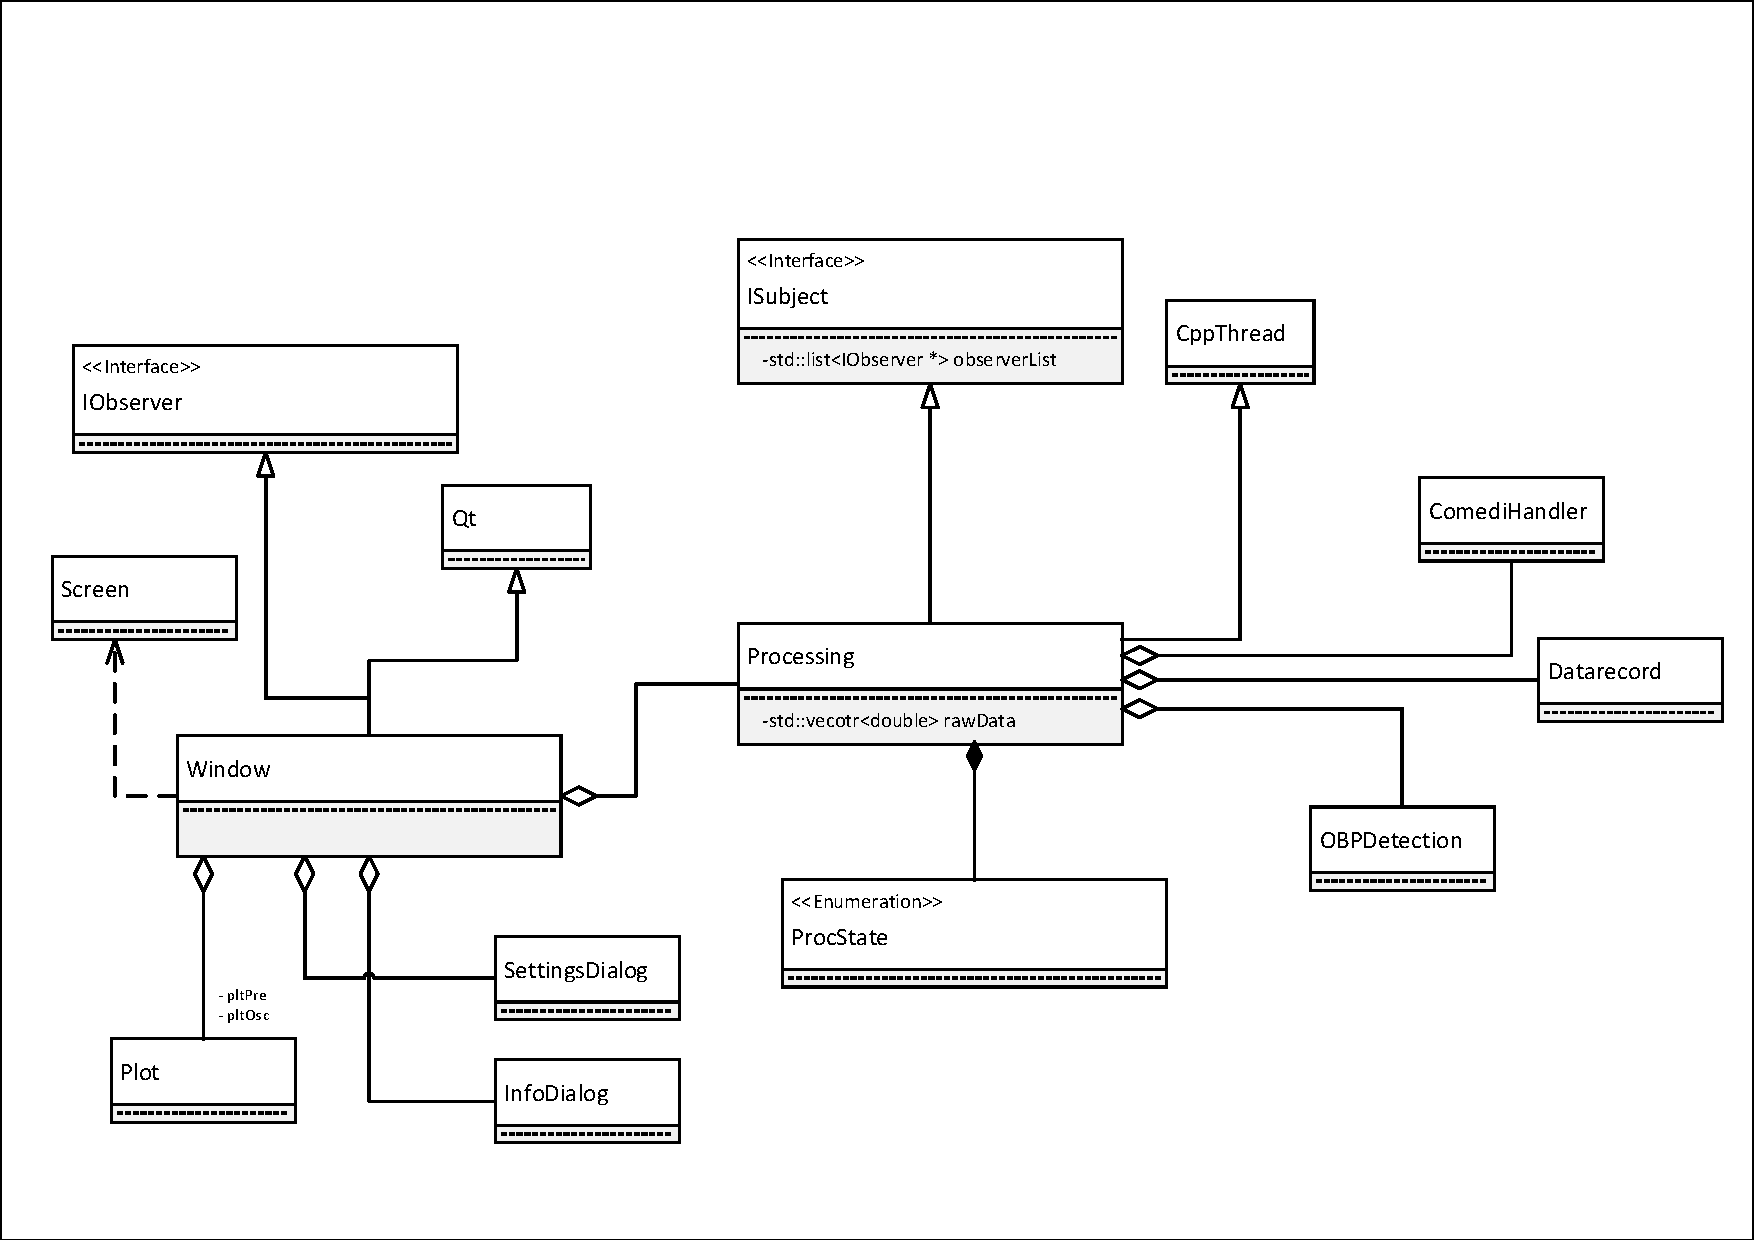
\includegraphics[width=\textwidth]{figures/cd2.pdf}
\caption{The Class Diagram. Needs work.}
\label{fig:CD}
\end{figure}

Communication between the  two main objects is done with callbacks in an observer pattern from the \mintinline{cpp}{Processing} to the \mintinline{cpp}{Window} class. The processing class is an observable subject that the window class can register to because it implements IObserver. The window has a reference to the processing class to pass on user input.

Following is a more in-depth discussion of the above mentioned elements.

\section{Data Processing}
In the processing class, the data is acquired and processed. The acquisition is handled by a ComediHandler object, that abstracts handling of the underlying hardware. The data is then filtered and the observers are notified so they can display the new data. 

The logic in the processing object is handled through a state machine. The OBPDetection class needs deflating pressure to extract the blood pressure characteristics from the oscillations. The state machine identifies this in the state 'Defalte'. The following section discusses the state machine in detail.

\subsection{State Machine}
Figure \ref{fig:sm} shows the state machine of the processing class. It is made up of an initial state (Config) that is only entered at start-up, an 'Idle' state and four states that are consecutively entered in an ideal measurement, called 'Inflate', 'Deflate', 'Empty' and 'Results'.

For every arriving sample, the state machine is executed according to the current state and potentially switched to another one. 

In every state, exept 'Config' the arriving sample is filtered and the results are sent to the observing objects. In the 'Inflate', 'Deflate' and 'Empty' states, the raw data is additionally recorded and ultimately saved as a file when exiting the 'Empty' state. 


\begin{figure}[ht]
\centering
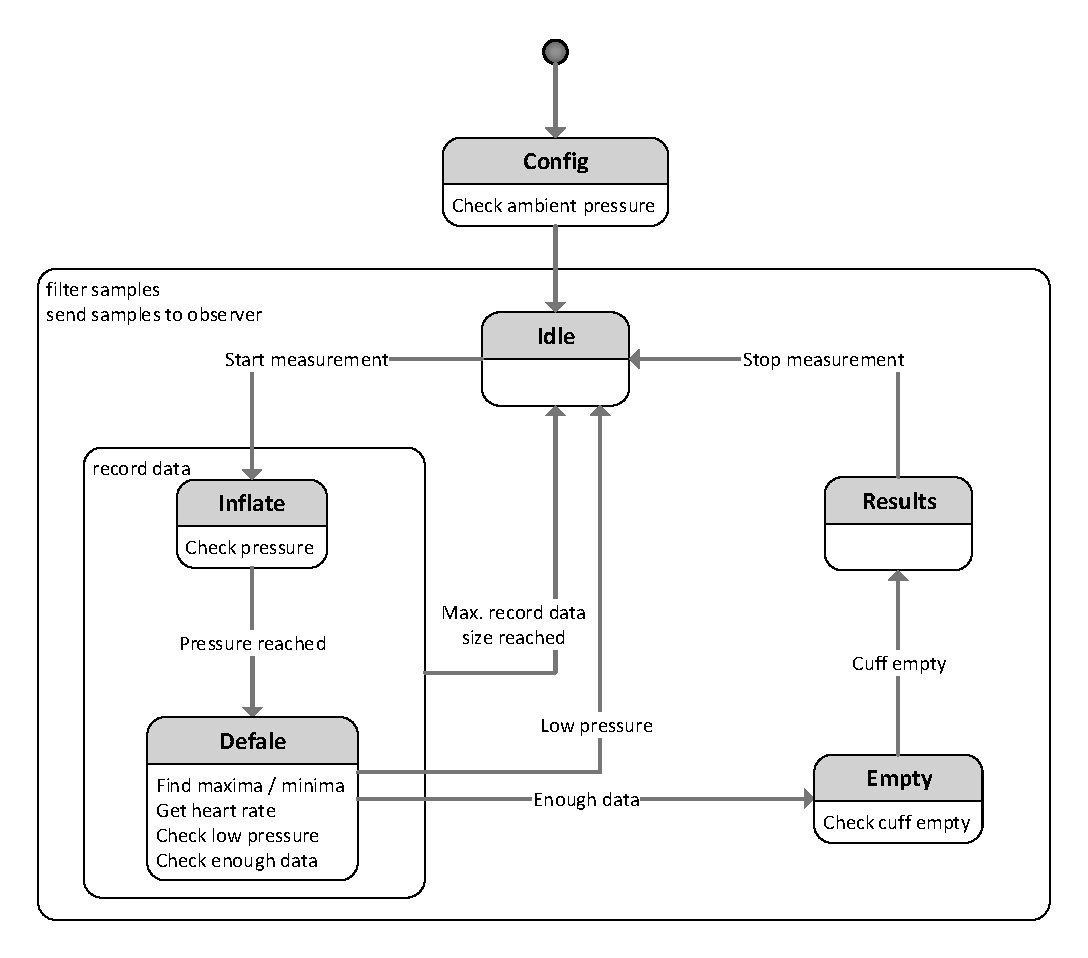
\includegraphics[width=\textwidth]{figures/state_machine.pdf}
\caption{The state machine implemented in the Processing class. Needs work.}
\label{fig:sm}
\end{figure}

\paragraph{Config} After a reset, the state machine starts in the 'Config' state, where the ambient voltage is registered. This is necessary, because the pressure sensor gives an absolute value, but pressure values are needed relative to atmospheric pressure. The raw pressure is read for \SI{250}{ms} and averaged. If that value has a deviation of less than \SI{1}{\milli\volt} to the maximal value, it is stored as ambient pressure and the state machine processes to the next state.

\paragraph{Idle} In the 'Idle' state, the processing class is waiting for the start of a measurement while filtering data and sending it to its observers. A measurement is externally triggered.

\paragraph{Inflate} While the pressure is below the configured pump-up pressure (default of \SI{180}{\mmHg}), in the 'Inflate' state, the raw data is recorded. When the pump-up pressure is surpassed, the state switches to 'Deflate'. In case the maximum data size for the recorded data is reached, the measurement is cancelled and the state switched to 'Idle'. Reaching the maximum data size takes \SI{5}{\minute} and should never happen during a measurement.

\paragraph{Deflate} In the 'Deflate' state, the data is fed into the OBPDetection object, which is described below in section \ref{sec:OBP}. This object decided when enough data is recorded and the progression to the 'Empty' state is possible. Alternatively, if the pressure falls below \SI{20}{\mmHg}, or the maximum data size is reached for the recorded data, the measurement is cancelled. 

\paragraph{Empty} This state is only needed to finish recording data until the pressure reaches zero. When this happens, the data is written to a file and the state is changed to 'Results'.

\paragraph{Results} After a successful measurement, in this state, the results are valid. Upon leaving this state, all results are reset and a new measurement can be started. The measurement can be cancelled externally from any of the previous states.  If the results state is never reached, the data will not be saved.


\subsection{Processing Class} 
The processing class inherits from the CppThread class and the ISubject class. CppThread is a wrapper to the std::thread class that was written by \citet{Porr2020Thread} to avoid static methods and makes the inheriting class a runnable thread. Processing has an instance of ComediHandler to acquire and two IIR filter instances to pre-process the data. The raw, unfiltered data is stored in a vector that can be handed to the Datarecord instance to save it as a file. Meanwhile, the filtered data is sent to the GUI to display and handed to the OPDetection instance that performs the algorithm. Data acquisition and filtering are happening whenever the thread is running, the state machine described above decides when data is passed to the OBPDetection or stored to a file. 

\subsubsection{Thread Safety}
The Processing class has public getter and setter methods, that allow objects, with access to it, to read and change configuration variables. These variables are defined as atomic, to make access to them thread-safe. Additionally, the configuration values can only be changed, when the thread is not running. This is a design choice, so a restart is necessary to apply changes and avoid changing the configuration mid-measurement. 

Similarly, the booleans set by starting and stopping the measurement and stopping the thread are atomic.

\subsection{ISubject}
ISubject is a simple interface defined in a header file that lets the implementing class notify its observers about certain events. Each notification is realised as a protected notify-X method. The public methods are 'attach' and 'detach'. Through these, a class that implements the below described IObserver (section \ref{sec:iobserver}) can be attached to the subject. This stores a reference to the object in a list. When one of the notify methods is called, the notification is sent to all the observers in the list. An observer can be removed through the detach method. 

The ISubject class can not be instantiated directly but has to be used to inherit from. This is achieved by having a protected constructor.


\subsection{Data Acquisition}
Access to the hardware is abstracted in the ComediHandler class. The class uses the comedi librairy (comedilib) \citep{comedi} to read data from the hardwae device. The ComediHandler is initialised when the Processing object is created. If the initialisation fails, e.g. because there is no device connected, the application terminates and an error message is printed.

Upon a successful startup, single samples can be read from the device either as a raw integer value or as a voltage value. Optionally, the whole buffer content can be read as raw values. The application is only reading voltage values.


\subsection{Filtering}
Two filters are used to process the acquired data as described in section \ref{sec:filt} above. The filter implementation was done by \citet{Porr2020iir}. The objects are initialised when the Processing class is created. They process data sample by sample as needed by a real-time application. Whenever a new sample is passed to them, a single filtered value is retruned. They are causual, so the order in which the samples are passed to it influences future outputs.


\subsection{OBPDetection}
The core algorithm is performed by the OBPDetection class. An object is initialised upon creation of the Processing class. The detailed description about what happens inside is provided above in the section \myref{sec:Deflation}. Configuration values that are stored in the OBPDetection class work correspondingly to the ones stored in the Processing class directly. They can be accessed through public getter and setter methods. This could be done anytime, but should only be done when no measurement is happening. If it is done during a measurement, the behaviour can not be guaranteed. 

The configuration values can only be set if they are within reasonable boundaries as defined in macros. However, a valid measurement is not guaranteed, if the values are changed from the default ones.

The data is passed to the object sample by sample like in the filters. Here, a pair of samples of pressure and oscillation data is always needed. The return value is a boolean which is true whenever a new maximum was detected in the oscillations. In this case, a new heart rate value can be read through the corresponding public method of the OBPDetection class. Additionally, the method should be checked that indicate when the measurement is finished. When the process is successfully done, the getter functions for the BP values, MAP, SBP and DBP will return valid values, otherwise they return $0.0$.

\subsection{Storing the Recorded Data}
The class Datarecord stores data in a file, given a file name. There are two options, one is to store it sample by sample, the other by handing it a vector of doubles to store. If the sampling rate is supplied, it will store the values with the corresponding time. Otherwise, with the corresponding sample number. In this application, the the data is stored at the end of a measurement, so a vector is handed to the object together with a file name that represents the current date and time. 


%
%\subsection{Project Setup and Compilation}
%The project is set up as a CMake project. Usually, Qt projects are set up using qmake (a .pro file), but CMake is supported as well. This application chose CMake because it is more powerful and allows integration with other tools, e.g. for continuous integration (CI). %TODO potentially include information about Travis CI (if set up)
%
%CMake ensures all required dependencies are installed as defined in the file CMakeList.txt and automatically generates a Makefile. This Makefile is used to build the project, linking all defined files and libraries.
%For example, this application requires the C++20 standard for the implemented algorithm. CMake generates an error when trying to build the application with a compiler that does not support C++20.



\section{User Interface}
The user interface is shown in figure \myref{fig:UI}. It is split up into two parts. The left side accepts user input and gives instructions to the user what they have to do to take their blood pressure. The right side shows the data being acquired in real-time. There are two plots. The upper plot shows pressure data filtered with a low-pass filter of \SI{10}{\Hz}, the lower plot shows the data additionally high-pass filtered at \SI{0.5}{\Hz}, which results in a bandpass filter. This is the oscillogram, the main input for the algorithm to determine the user's blood pressure.

\begin{figure}
\centering
%
\includegraphics[scale=0.125]{GlaLogo.pdf}
\caption{UI}
\label{fig:UI}
\end{figure}

As mentioned above, the graphical user interface (GUI) is built with Qt.
The QtDesigner was used to design a first draft of the GUI, but because this does not allow integration into applications that are built outside of the Qt development environment, the whole GUI was completely built in C++ code from this draft.

\subsection{Guided Blood Pressure Measurement}
The left side of the GUI guides the user through taking blood pressure. The process is split up into five pages that are shown in figure \ref{fig:UIguide}.  All pages have a dial that shows the current pressure in \SI{}{\mmHg}. The first page has information on how to prepare for the measurement. Pressing the button at the bottom of the page starts the measurement process. The button is only enabled if the processing part of the application is ready.

\begin{figure}[ht]
\centering
%
\includegraphics[scale=0.125]{GlaLogo.pdf}
\caption{The screens that guide the user through taking their blood pressure in the order that they are shown.}
\label{fig:UIguide}
\end{figure}

The second page instructs the user to pump up the pressure in the cuff to a certain value. The default value is \SI{180}{\mmHg}. Once that value is reached, the GUI automatically switches to the next page.

This page tells the user to release the pressure in the cuff again. This should be done slowly at a rate of approximately \SI{3}{\mmHg/\second}. There is no other feedback than the dial for how fast the pressure is being released. At the bottom of the page, the current heart rate, calculated from the latest oscillation peaks, is shown.

Once enough data is collected, the fourth page is shown. It requires the user to deflate the cuff completely to show the results. If the algorithm fails to collect enough data within a specified time (configured as \SI{5}{\minute}) the measurement stops and goes back to the start page.

When the pressure in the cuff reaches nearly zero, the results page is shown. It displays MAP, SBP, DBP and the average heart rate during the measurement. All data is shown as whole numbers without decimals. 

\subsection{Menu}
A menu bar provides access to an information pane as well as a settings pane. Both open up as dialogue windows and disable user input on the main window. Data acquisition is kept running and is displayed in the plots.

\subsubsection{Information}
The information pane shows the application version number, the licence and provides a link to the project GitHub page. Figure \ref{fig:UIinfo} shows the dialogue.

\begin{figure}[ht]
\centering
%
\includegraphics[scale=0.125]{GlaLogo.pdf}
\caption{The information dialogue.}
\label{fig:UIinfo}
\end{figure}


\subsubsection{Settings}
The settings dialogue (shown in figure \ref{fig:UIsettings}) lets the user change some application configurations. The user is not recommended to change these if they are not aware of the consequences. The settings are stored persistently but only take effect after restarting the application. The range of accepted values is limited, to keep the algorithm working. Because not all values have been tested, the user is warned that the application might not perform reliably anymore. The values are stored once the user presses the 'OK' button. If the 'Cancel' button is clicked, the settings application is closed without saving the values.

The values can be reset by pushing the corresponding button. These changes take effect immediately. 

\begin{figure}[ht]
\centering
%
\includegraphics[scale=0.125]{GlaLogo.pdf}
\caption{The settings dialogue.}
\label{fig:UIsettings}
\end{figure}

The handling and storing of these values is done through the QSettings class of the Qt library. It allows to save and load values by specifying a string key. If there is no key found with the provided name, the default value is selected. The default value is what is hard-coded in the Processing class.

\subsection{The Window Class}
The \mintinline{cpp}{Window} class inherits from the \mintinline{cpp}{QMainWindow} class and the \mintinline{cpp}{IObserver} class. The \mintinline{cpp}{QMainWindow} class makes the class an executable Qt window, with Qt taking care of updating the GUI and generating events for button clicks and so on. The \mintinline{cpp}{IObserver} makes the class able to be registered as an observer for a subject that will send notifications to the observer. More on the \mintinline{cpp}{IObserver} below.

All GUI elements are set up in the constructor of  \mintinline{cpp}{Window}, including the settings and info plane. However, they will only be shown if necessary. E.g. what page of the user instructions is shown is defined by the setting of the screen enum (currentScreen).

The Window object is instantiated with a reference to a Processing object in the constructor. This is necessary so the user inputs can be relayed and the Processing thread can be stopped when the window is closed and the application exited. 

\subsection{The IObserver Class}
The \mintinline{cpp}{IObserver} class defines the functions that the observable class (the subject) uses to notify the observer. All functions are virtual but implemented as empty functions. This way, the observing class can choose to implement and therefore listen to the notifications that it wants to and ignore the ones that it does not. 

Just like the ISubject class, the IObserver class can not be instantiated directly but has to be used to inherit from. 

\paragraph{The following methods can be implemented:}
\setlist{nolistsep}
\begin{itemize}[noitemsep]
\item Ready: \newline
Informs the observer that the subject is ready.
\item New Data: \newline
Sends a new data pair to the observer. Each data pair consists of pressure data and oscillation data. Both are doubles.
\item Switch Screen: \newline
Tells the observer which screen to display.
\item Results: \newline
Sends the results to the observer. The results are three doubles for MAP, SBP and DBP.
\item Heart Rate: \newline
Sends a new heart rate value to the observer. The value is a double.
\end{itemize}

These methods are called from a class that inherits from ISubject, which is explained in detail in section \ref{sec:isubject} below. 

\subsubsection{Thread safety}
Because the methods from the \mintinline{cpp}{IObserver} class are called from an object, which is likely to be running in another thread than the window, it is important to implement all functions in a thread-safe manner. Qt offers a good way to do this by sending queued events. 

One example of how to enable the start button, in a not thread-safe way is by accessing it directly, as follows: 

\begin{minted}[breaklines]{cpp}  
btnStart->setDisabled(false);
\end{minted}

Instead, the function \mintinline{cpp}{QMetaObject::invokeMethod} is called to send an event to the GUI thread. This is done by specifying the object, which function of the object to call, what arguments to set, and the type of event to send. The \mintinline{cpp}{Qt::QueuedConnection} will send an event into a queue that will be handled when the thread is executed. The function to call is given as a string argument. Considering the example above, this results in the following statement:

\begin{minted}[breaklines]{cpp}  
bool bOk = QMetaObject::invokeMethod(btnStart, "setDisabled", Qt::QueuedConnection,  Q_ARG(bool, false));
assert(bOk);
\end{minted}

The return value confirms if the connection could be made, i.e. the given string is a valid function to call for the given object. This is tested through an assert during development. The assert will fail if the boolean is not true. It is important not to have the assert around the whole function call, because it will be removed in the release build. 

The plots have their underlying data set changed every time a new sample is available because a new sample is always added on the right side and an old one is discarded on the left side. This is made by changing the raw data in memory and therefore, the Qt process is not informed about that. To solve this issue, the plots are regularly updated manually. This happens in a timer event with an interval of 50 ms, which is enough for the human eye to see a continuous movement. To avoid thread safety problems, the plot objects are accessed after acquiring a mutex.


%TODO \section{Settings}
\section{Third Party Software}

The following third party software is used in the developed application:

\begin{itemize}
\item Qt %TODO ref
\item CppThread a wrapper to the std::thread class written by Bernd Porr to avoid static methods. %TODO ref
\item \emph{iir1} An implementation of the infinite impulse response (IIR) filters for sample-by-sample, real-time processing written in C++ by Bernd Porr. Provided as a library.%TODO ref
\item \emph{plog} Portable, simple and extensible C++ logging library. %TODO ref
\item \emph{comedilib} 
\end{itemize}

